\documentclass[12pt]{article}
\usepackage{caption}
\usepackage{graphicx}
\usepackage{hyperref}
\usepackage{amsmath}
\hypersetup{%
    pdfborder = {0 0 0}
}
\hypersetup{
    colorlinks,
    citecolor=blue,
    filecolor=blue,
    linkcolor=blue,
    urlcolor=blue
}
\renewcommand{\familydefault}{\sfdefault}
\renewcommand{\captionfont}{\small}

\author{Bernd Porr}
\title{Deep learning}

\begin{document}

\maketitle

\section{Inductive learning with Deep Learning}
We have a dataset $\vec{x}_1, \ldots, \vec{x}_N$ which should be converted
via the function
\begin{equation}
  \vec{y}=f(\vec{x}) \label{inductive}
\end{equation}
into $\vec{y}$.  The goal is to learn this function with the help of
examples $\vec{x}_1,\vec{y}_1$; $\vec{x}_2,\vec{y}_2; \ldots$.

The following sections show how learning of $f$ with the help
fo examples can be achieved. This is called ``inductive learning''.

\section{Linear neuron}

\begin{figure}[!hbt]
\begin{center}
\mbox{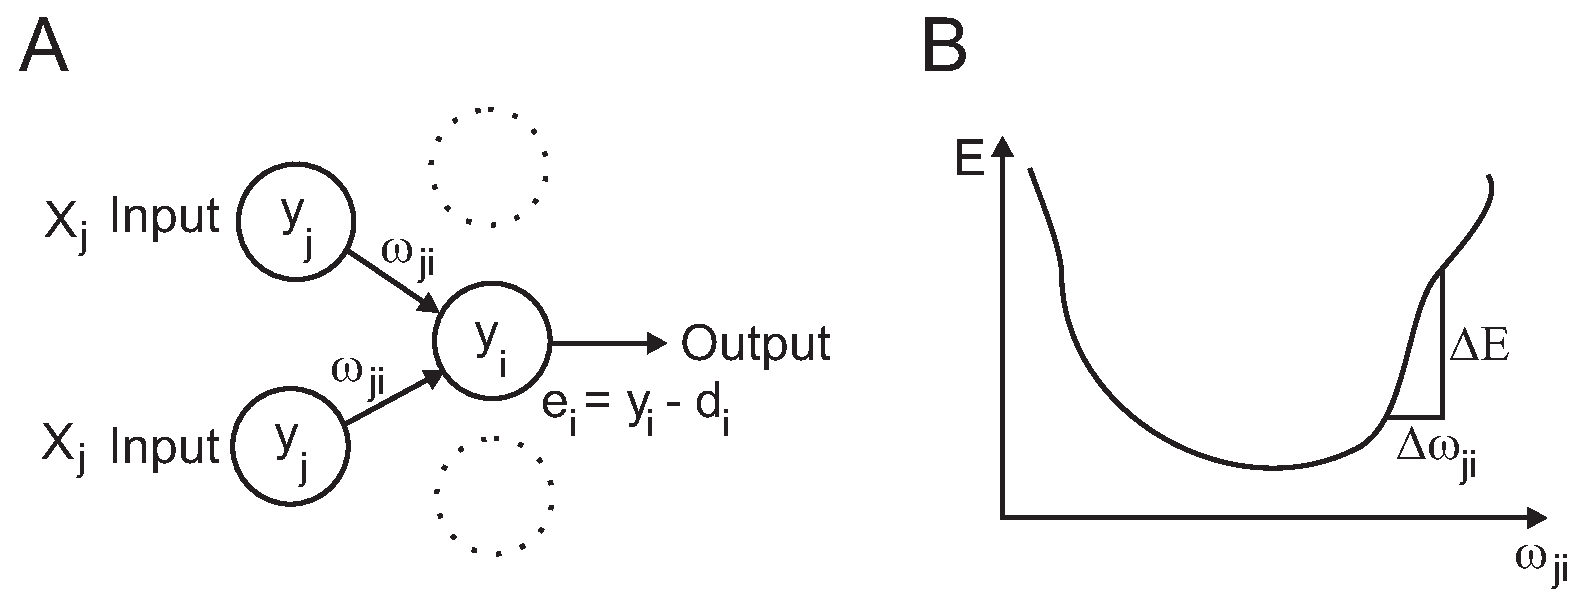
\includegraphics[width=\textwidth]{one_layer}}
\end{center}
\caption{Simple linear neuron
\label{one_layer}}
\end{figure}

Fig.~\ref{one_layer}A shows a neuron in a single layer.
Its activation is $y(n)$ and is the $i$th neurn in this layer.
$n$ is the current time-stamp. The input activity to the neuron $x_j(n) =
y_j(n)$ is weighted by $\omega_{ji}$ and summed up to:
\begin{equation}
  y_i(n) = \sum_j y_j(n) w_{ji} \label{linear_sum}
\end{equation}
Our function $f$ from the introduction is here a simple linear
combination of input activities where $\omega_{ji}$ had to be learned
to approximate $f$.

\section{The error signal}
The task is to learn a function $f$ which converts the input activities to output activities
(Eq.~\ref{inductive}).
This is achived by minimising the error:
\begin{equation}
  e_i(n) = y_i(n) - d_i(n) \label{output_error}
\end{equation}
where $d_i(n)$ is the desired output value and $y_i(n)$ the actual output value.
The goal is to minimise the square of the error:
\begin{equation}
  E = \frac{1}{2} e^2 \label{quaderr}
\end{equation}

\section{Gradient descent}
The central trick here is to take the partial derivative in respect to the weights $\omega_{ji}$
\begin{eqnarray}
  \Delta\omega_{ji} & = & - \mu \frac{\partial E}{\partial \omega_{ji}} \label{graddes} \\
  \omega_{ji} & \leftarrow & \omega_{ji} + \Delta\omega_{ji}
\end{eqnarray}
Why does this make sense? Fig.~\ref{one_layer}B shows the relationship
between the error $E$ and the weight $\omega_{ji}$. In this example if
the weight is slightly increased the squared error is also increased
which is not desirable.  However, if increasing $\omega_{ji}$ reduces
the squared error $E$ then it's a good idea to keep changing the
weight in this direction. This approach is called \textsl{gradient
  descent}.

\section{Learning rule for the single layer}
We can now derive the learning rule which changes the weights
$\omega_{ji}$.  We simply insert Eq.~\ref{linear_sum},
\ref{output_error} and \ref{quaderr} into Eq.~\ref{graddes}:
\begin{eqnarray}
  \Delta\omega_{ji}
   & = & - \mu \frac{1}{2} \frac{\partial ( d_i(n) - y_i(n) )^2 }{\partial \omega_{ji}} \\
   & = & - \mu \frac{1}{2} \frac{\partial \left( d_i(n) - \sum_j y_j(n) w_{ji} \right)^2 }{\partial \omega_{ji}} \\
  & = & \mu \underbrace{\left(d_i(n) - \sum_j y_j(n) w_{ji}\right)}_{-e_i(n)} \cdot y_j(n) \\
   & = & - \mu \underbrace{\frac{\partial E}{\partial y_i}}_{-e_i(n)} \underbrace{\frac{\partial y_i}{\partial \omega_{ji}}}_{y_j(n)} \label{chainrule}\\
  & = & \mu \cdot e_i(n) \cdot y_j(n) \label{learningrule}
\end{eqnarray}
where $\mu << 1$ is the learning rate or the ``step change''. The
learning rule Eq.~\ref{learningrule} is simply a multiplication of the
input activity $y_j(n)$ with the error $e_i(n)$.


\section{Multi-layer network: error backpropagation and learning rule}
\begin{figure}[!hbt]
\begin{center}
\mbox{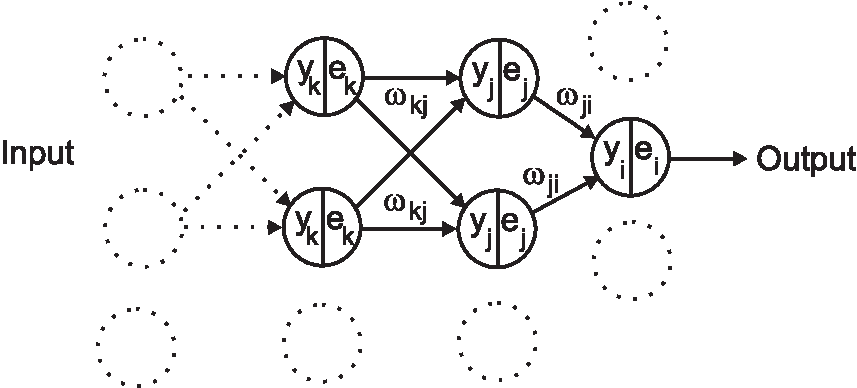
\includegraphics[width=\textwidth]{multi_layer}}
\end{center}
\caption{Mehrschichtiges Feedforward Netz
\label{multi_layer}}
\end{figure}

Fig.~\ref{multi_layer} shows now a network with multiple layers.
The forward progression of the signals $y_j$ from the input to
the output and follows exactly the same recipe as for the single
layer network above using Eq.~\ref{linear_sum}.
Also the error $e_i$ at the output layer can simply be calculated
as the difference between the actual output $y_i$ and the desired output $d_i$ (see
Eq.~\ref{output_error}). The problem is how to calculate the
internal errors $e_j$ und $e_k$ and how they change the hidden weights $\omega_{kj}$
(see Eq.~\ref{chainrule}):
\begin{equation}
  \frac{\partial E}{\partial \omega_{kj}} = \underbrace{\frac{\partial E}{\partial y_j}}_\textrm{trick!} \frac{\partial y_j}{\partial \omega_{kj}}
  \label{gradint}
\end{equation}
The central trick here is to express $\frac{\partial E}{\partial y_j}$
with the help of the activities $y_i$ at the output und then to
identify the resulting terms with our linear sum Eq.~\ref{linear_sum}
and the chain rule Eq.~\ref{chainrule}:
\begin{equation}
  \frac{\partial E}{\partial y_j} = \sum_i \underbrace{\frac{\partial E}{\partial y_i}}_{-e_i} \cdot \underbrace{\frac{\partial y_i}{\partial y_j}}_{\omega_{ji}} \label{dltrick}
\end{equation}
Eq.~\ref{dltrick} is again substituted into Eq.~\ref{gradint} which gives us:
\begin{equation}
  \frac{\partial E}{\partial \omega_{kj}} = - \left( \sum_i e_i \omega_{ji} \right) \frac{\partial y_j}{\partial \omega_{kj}}
  \label{gradintback}
\end{equation}
with
\begin{equation}
y_j = \sum_k y_k(n) w_{kj}
\end{equation}
and leads to:
\begin{eqnarray}
  \frac{\partial E}{\partial \omega_{kj}} & = & - \left( \sum_i e_i \omega_{ji} \right) \underbrace{\frac{\partial \left(\sum_k y_k(n) w_{kj}\right)}{\partial \omega_{kj}}}_{y_k} \\
                                         & = & - \left( \sum_i e_i \omega_{ji} \right) y_k
\end{eqnarray}
The change of the internal weight $\omega_{kj}$ leads then to:
\begin{equation}
\Delta\omega_{kj} = \mu \cdot y_k \cdot \underbrace{\sum_i e_i \omega_{ji}}_{e_j}
\end{equation}
where $e_j$ is the internal error and we can now use this recipe to
calculate all internal errors.  This is called \textsl{error
  backpropagation} which now allows to establish networks with an
arbitrary number of layers.

\begin{figure}[!hbt]
\begin{center}
\mbox{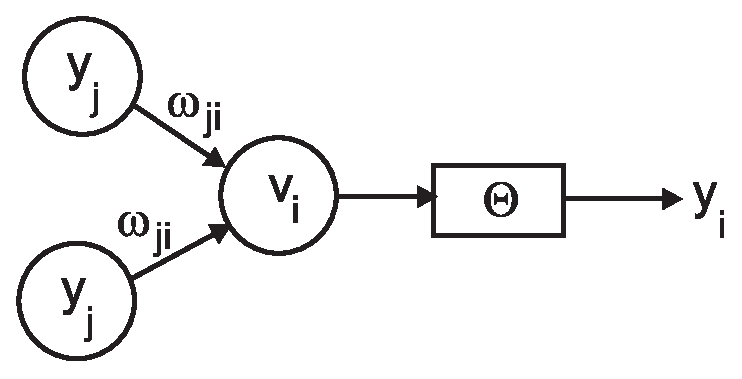
\includegraphics[width=0.5\textwidth]{nonlin}}
\end{center}
\caption{Neuron mit nichtlinearer Characteristik
\label{nonlin}}
\end{figure}

\section{Non-linear networks}
Only if computations in the separate neurons are non-linear
deeper networks make sense. Any linear deep network could always be
reduced to a single layer network rendering any deeper network
pointless. Consequently, we need to introduce now non-linearities.
Fig.~\ref{nonlin} shows a non-linear neuron which is the central building block
of any deep network where after the linear summation we introduce a non-linearity $\Theta$
which we call activation function:
\begin{equation}
  y_i(n) = \Theta\left(\underbrace{\sum_j y_j(n) w_{ji}}_{v_i} \right) \label{nonlinear_sum}
\end{equation}

The crucial question is if the introduction of the activation function
changes the learning rule. Luckily not much.
Looking at Eq.~\ref{chainrule} it becomes directly clear that the
chain rule is simply expanded by another term:
 \begin{equation}
 \frac{\partial E}{\partial \omega_{ji}}  = \frac{\partial E}{\partial y_i} \underbrace{\frac{\partial y_i}{\partial v_i}}_{\Theta^\prime} \frac{\partial v_i}{\partial \omega_{ji}}
 \end{equation}
 where $\Theta^\prime$ is simply the derivative of the activation function $\Theta$. Consequently the
 weight change at the output is now calculated as:
\begin{equation}
  \Delta\omega_{ji} = \mu \cdot \Theta^\prime(y_i) \cdot y_j \cdot e_i 
\end{equation}
and the internal error as:
\begin{equation}
\Delta\omega_{kj} = \mu \cdot \Theta^\prime(y_j) \cdot y_k \cdot \underbrace{\sum_i e_i \omega_{ji}}_{e_j} 
\end{equation}

Strictly, the activation function needs to be differentiable. However,
it turned out that the one way rectifier (Rectifiying Linear Unit = ReLU)
works extremely well:
\begin{equation}
  \Theta(v) =
  \begin{cases}
    0, & \text{if}\ v < 0 \\
    v, & \text{otherwise}
  \end{cases}
\end{equation}
Its derivative has no definite solution at its origin so that one needs
to decide if the derivative is zero there or one.
Other popular activation functions are $\Theta(v)=\tanh(v)$ or $\Theta(v)=\frac{1}{1+e^{-v}}$.




\end{document}
